\section{Impact of accretion}\label{sec:accretion}

In this section, I compare models  1 \& 4 listed in \cref{tab:simulations_settings}, which correspond to the maximum and minimum accretion case, respectively. Here, I examine the effects of accretion on the evolution of the system.

In \cref{sec:mass_transfer_RLOF}, I showed that periodic variations are naturally integrated in my models due to the outer orbit's eccentricity. The key point though, is that the timescale of this periodicity is equal to the period of the outer orbit. In the parent and next section, I focus on the global evolution of the orbital parameters. As a result, the presented graphs associated with the outer orbit, display not only the original output of my simulations, but also smoothed versions of it with a width equal to $3 \times P_{out}$. The is for illustration purposes only, as it is easier for the reader to follow the comparison between the models listed in \cref{tab:simulations_settings}. 

\subsection{Outer orbit}

In \cref{fig:accretion_outer_semimajor_axis}, \cref{fig:accretion_outer_ecc} and \cref{fig:accretion_inc}, I display the evolution of the semi-major axis, eccentricity and the inclination of the outer orbit relative to the inner orbit, respectively.

For the minimum accretion case, the outer orbit decays faster, see \cref{fig:accretion_outer_semimajor_axis}. This behavior is expected, because more mass is lost from the system and the ejected mass carries away orbital angular momentum. Furthermore, as the tertiary approaches the inner binary, tidal effects between the two orbits become stronger. Tides tend to circularize and flatten the outer orbit. More specifically, in the equilibrium-tide model, the circularization timescale is $\propto \frac{R_{\star}}{\alpha}^{-8}$ and the faster decay of the orbit leads to a faster circularization too, see \cref{fig:accretion_outer_ecc}. Finally, in both cases, the outer orbit, which is already coplanar with the inner orbit, remains close to coplanarity, see \cref{fig:accretion_inc}.
\begin{figure}[!htb]
    \centering
    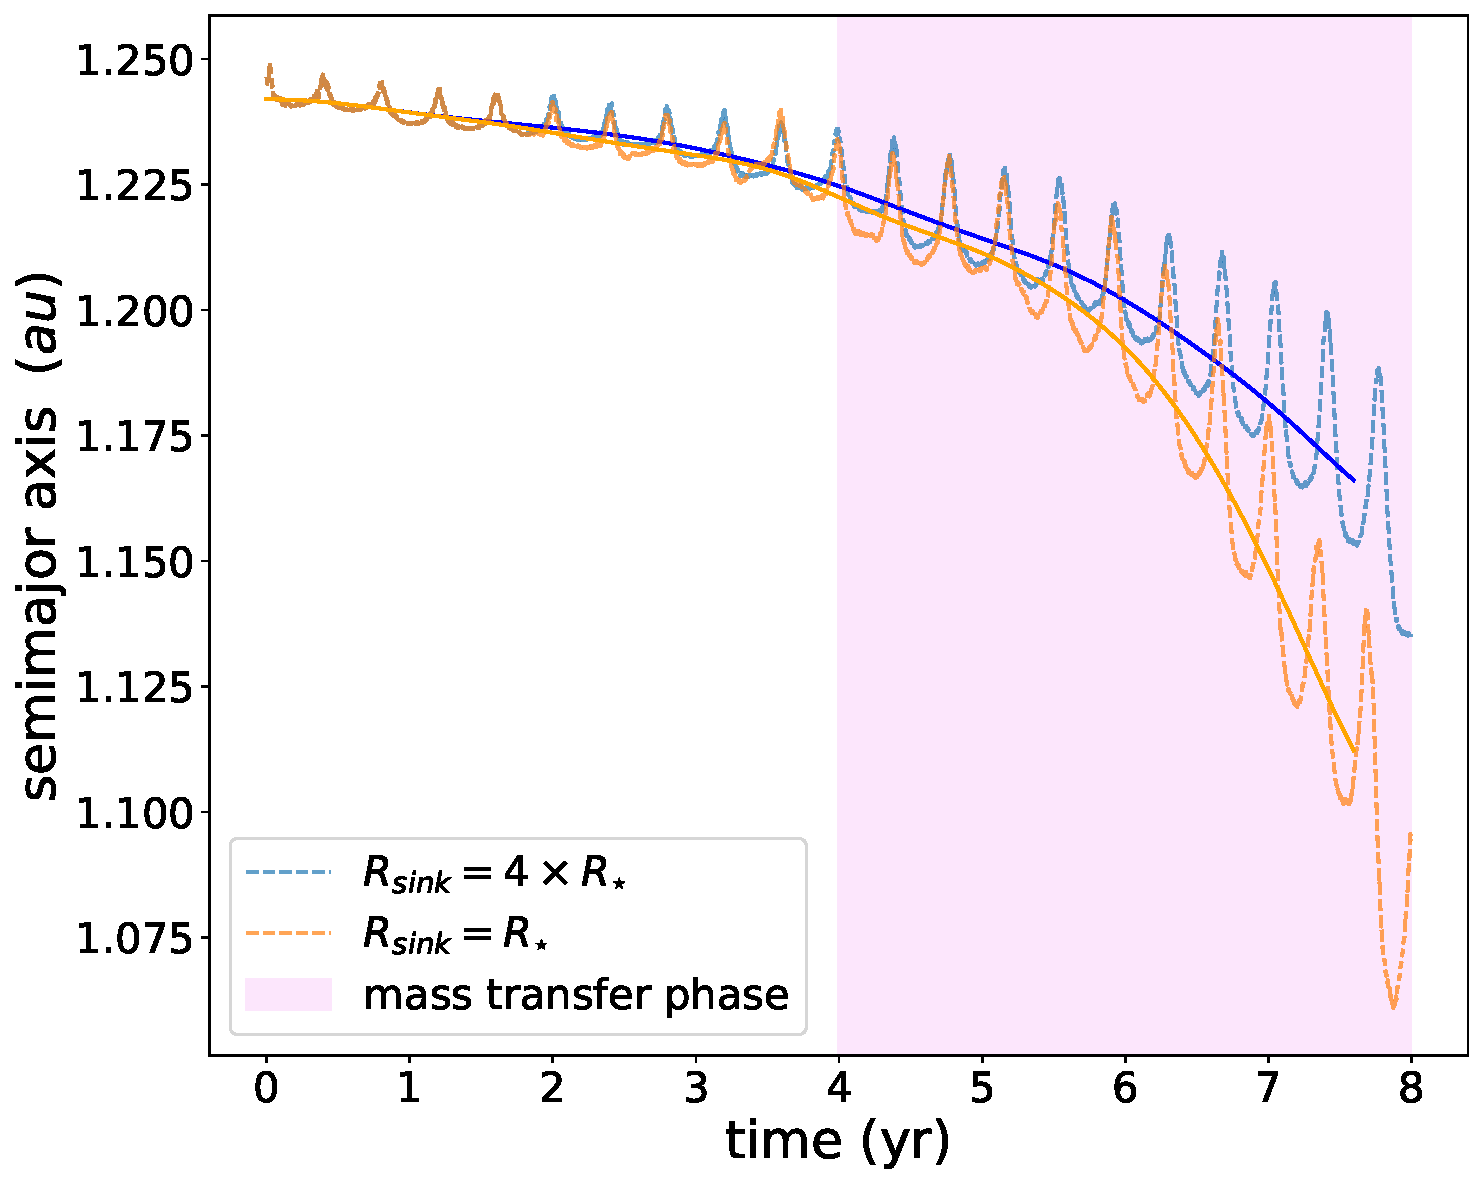
\includegraphics[width=0.85\textwidth]{Thesis/graphs/accretion_case/accretion_outer_semimajor_axis.pdf}
    \caption{Evolution of the semi-major axis of the outer orbit for the minimum and maximum accretion case. The simulated data is shown in dashed lines. The continues lines are smooth representations of the simulated data in their respective colors. The last three orbits are not included in the smoothed version, because the lack of data above $8$ yr will erroneously flatten the slopes.}
    \label{fig:accretion_outer_semimajor_axis}
\end{figure}
\begin{figure}[H]
    \centering
    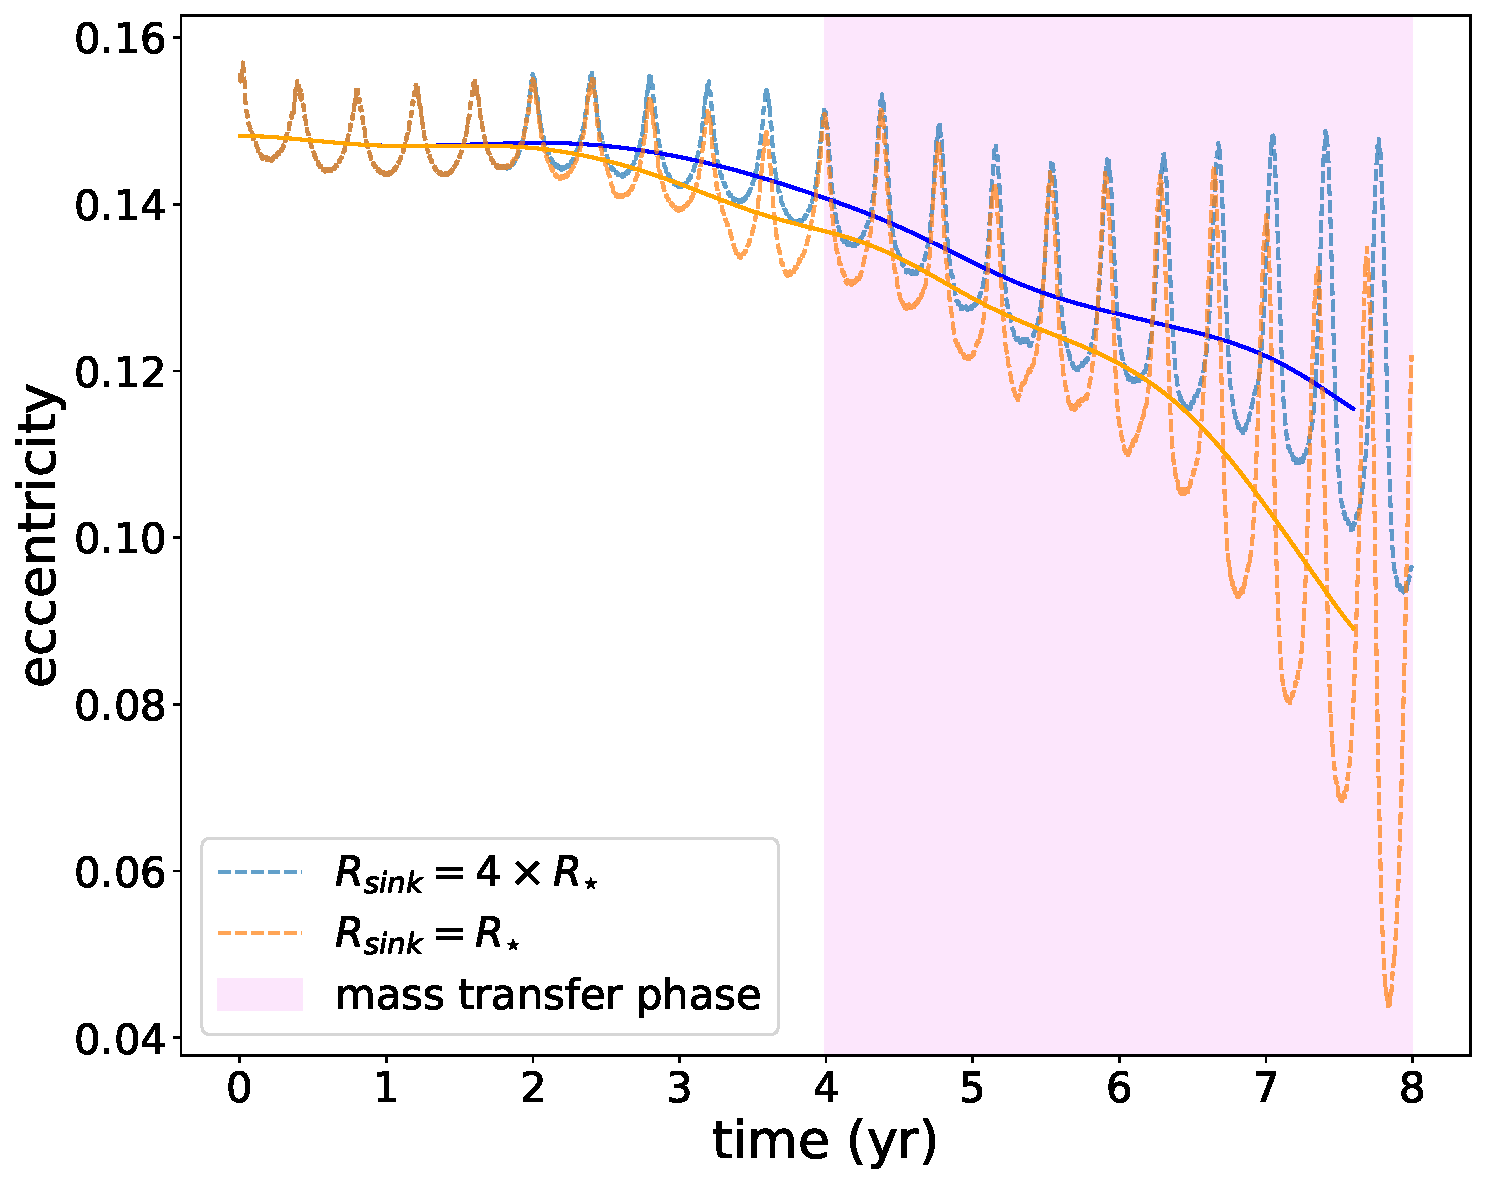
\includegraphics[width=0.85\textwidth]{Thesis/graphs/accretion_case/accretion_outer_ecc.pdf}
    \caption{Evolution of the eccentricity of the outer orbit for the minimum and maximum accretion case. The simulated data is shown in dashed lines. The continues lines are smooth representations of the simulated data in their respective colors. The last three orbits are not included in the smoothed version, because the lack of data above $8$ yr will erroneously flatten the slopes.}
    \label{fig:accretion_outer_ecc}
\end{figure}
\begin{comment}
\begin{figure}[H]
    \centering
    \begin{subfigure}{.5\textwidth}
    \centering
    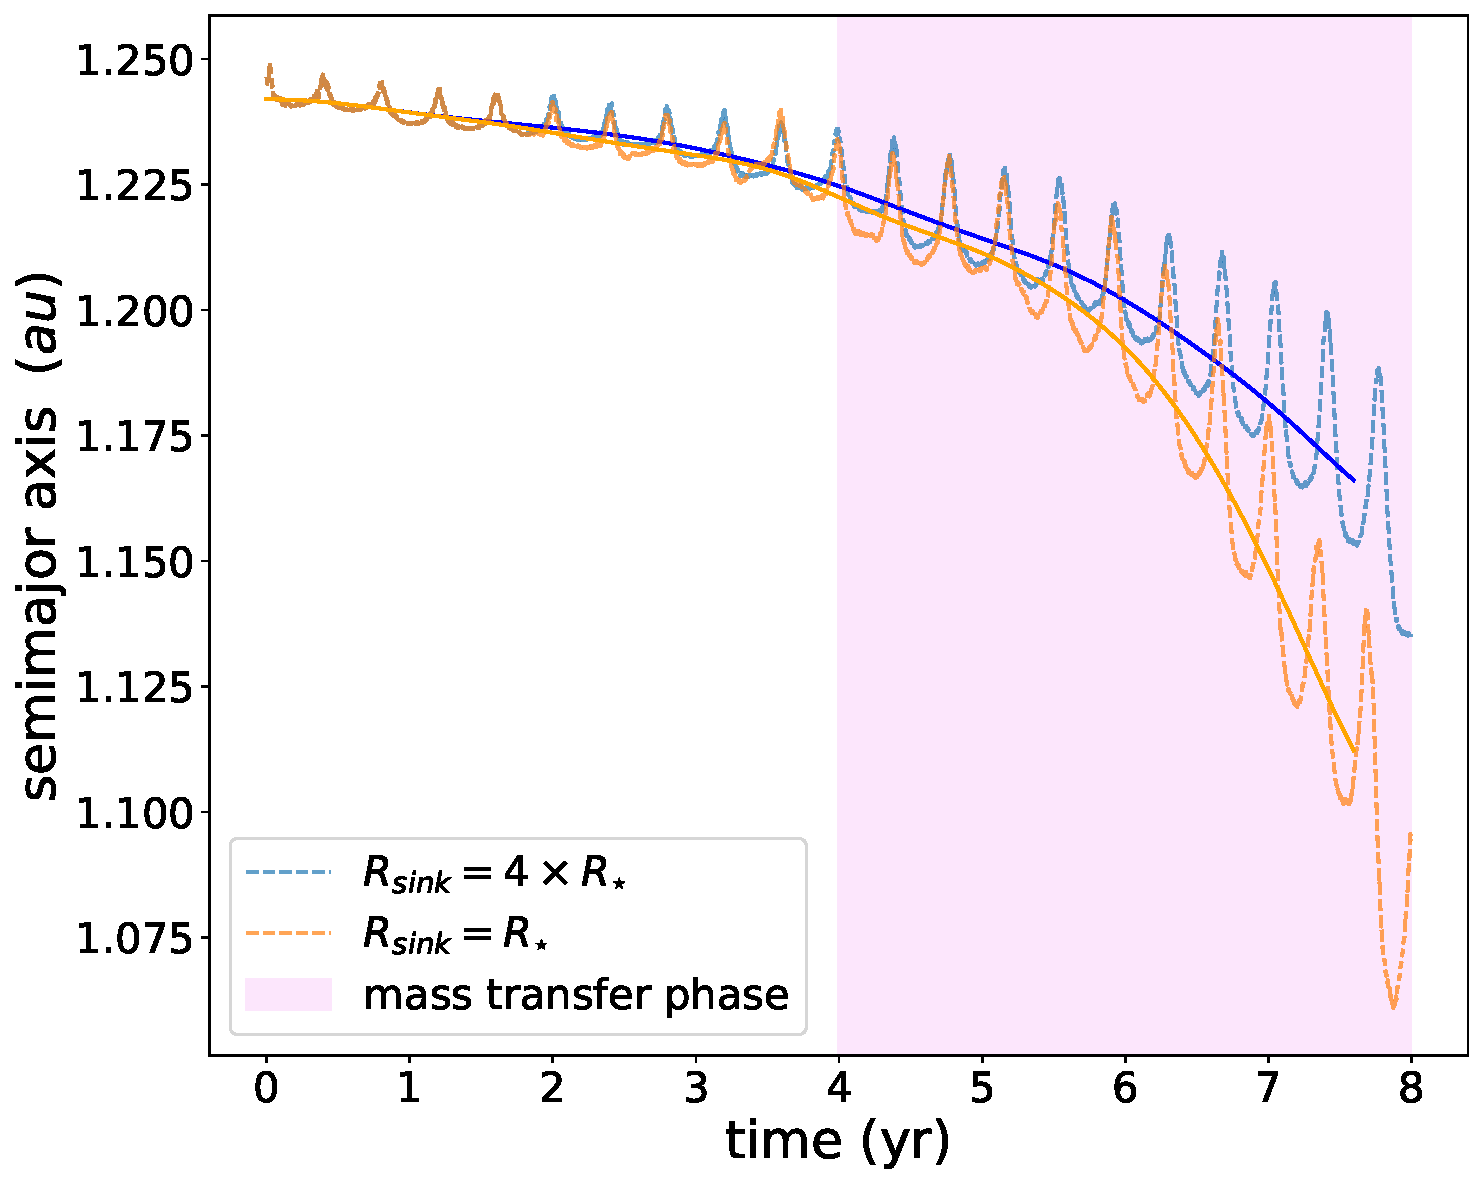
\includegraphics[width=0.9\textwidth]{Thesis/graphs/accretion_case/accretion_outer_semimajor_axis.pdf}
    \end{subfigure}%
    \begin{subfigure}{.5\textwidth}
    \centering
    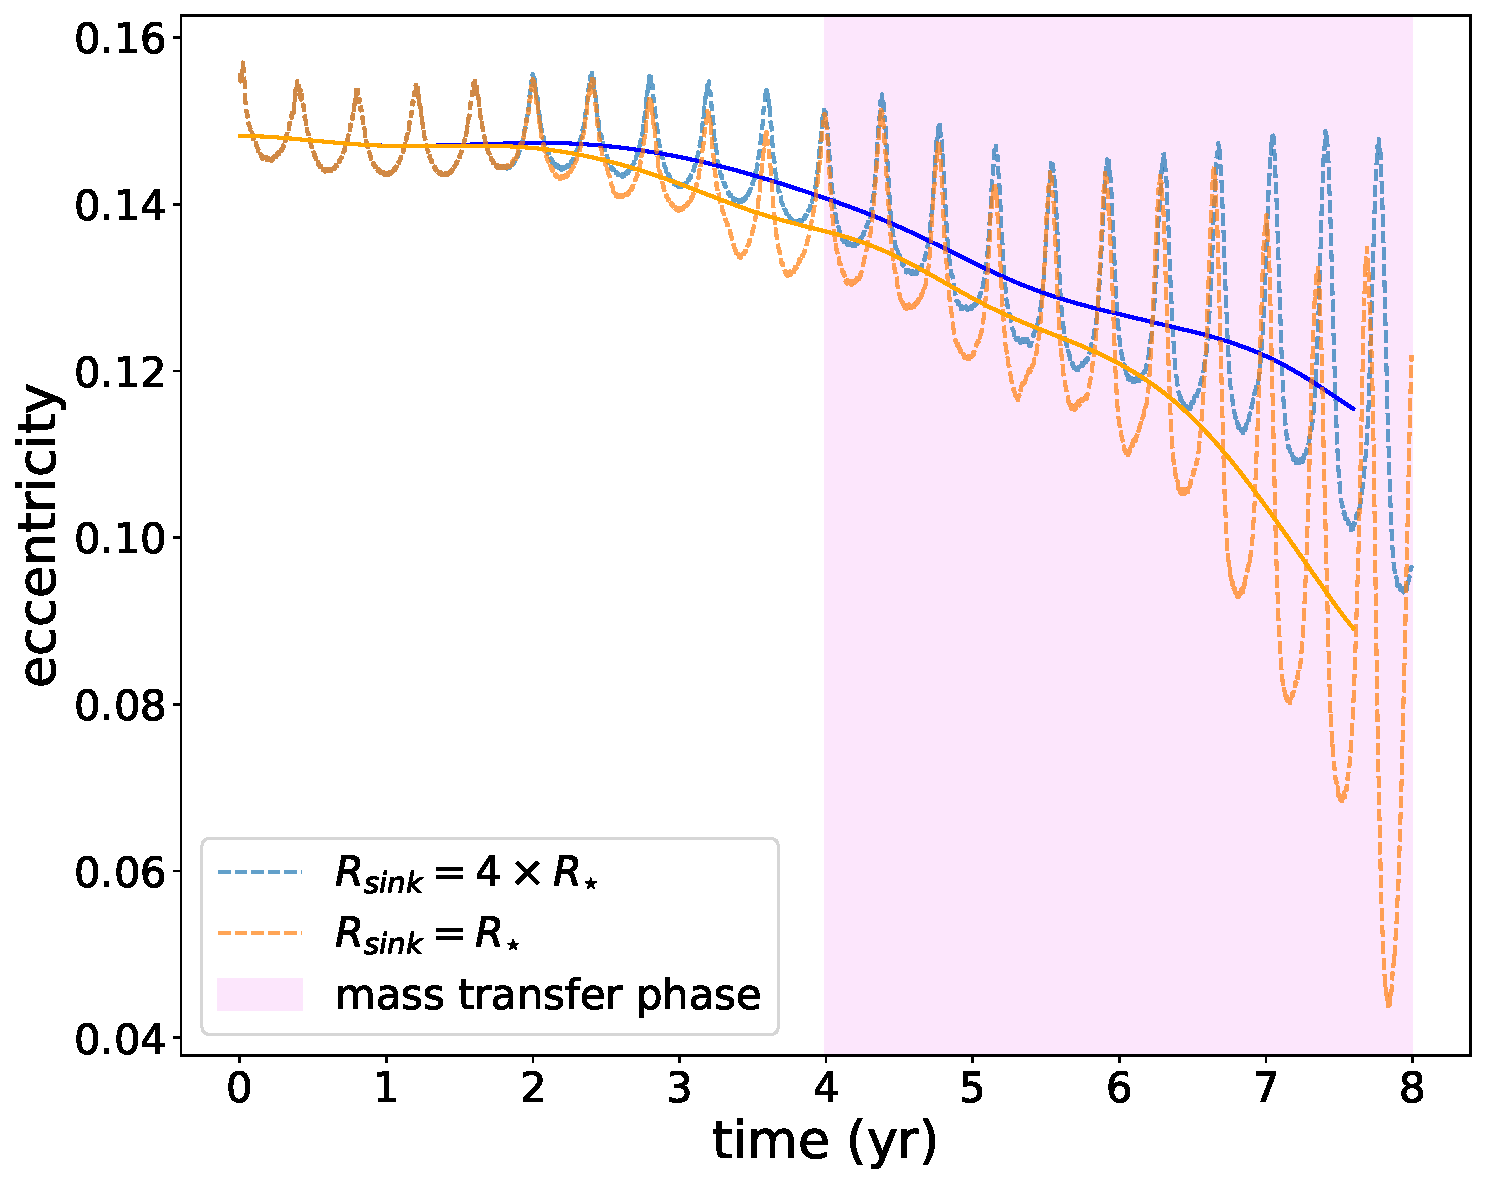
\includegraphics[width=0.9\textwidth]{Thesis/graphs/accretion_case/accretion_outer_ecc.pdf}
    \end{subfigure}
    \caption{ Evolution of the semi-major axis (left) and eccentricity (right) of the outer orbit}
    \label{fig:acc_outer_orbit}
\end{figure}
\end{comment}
\begin{figure}[H]
    \centering
    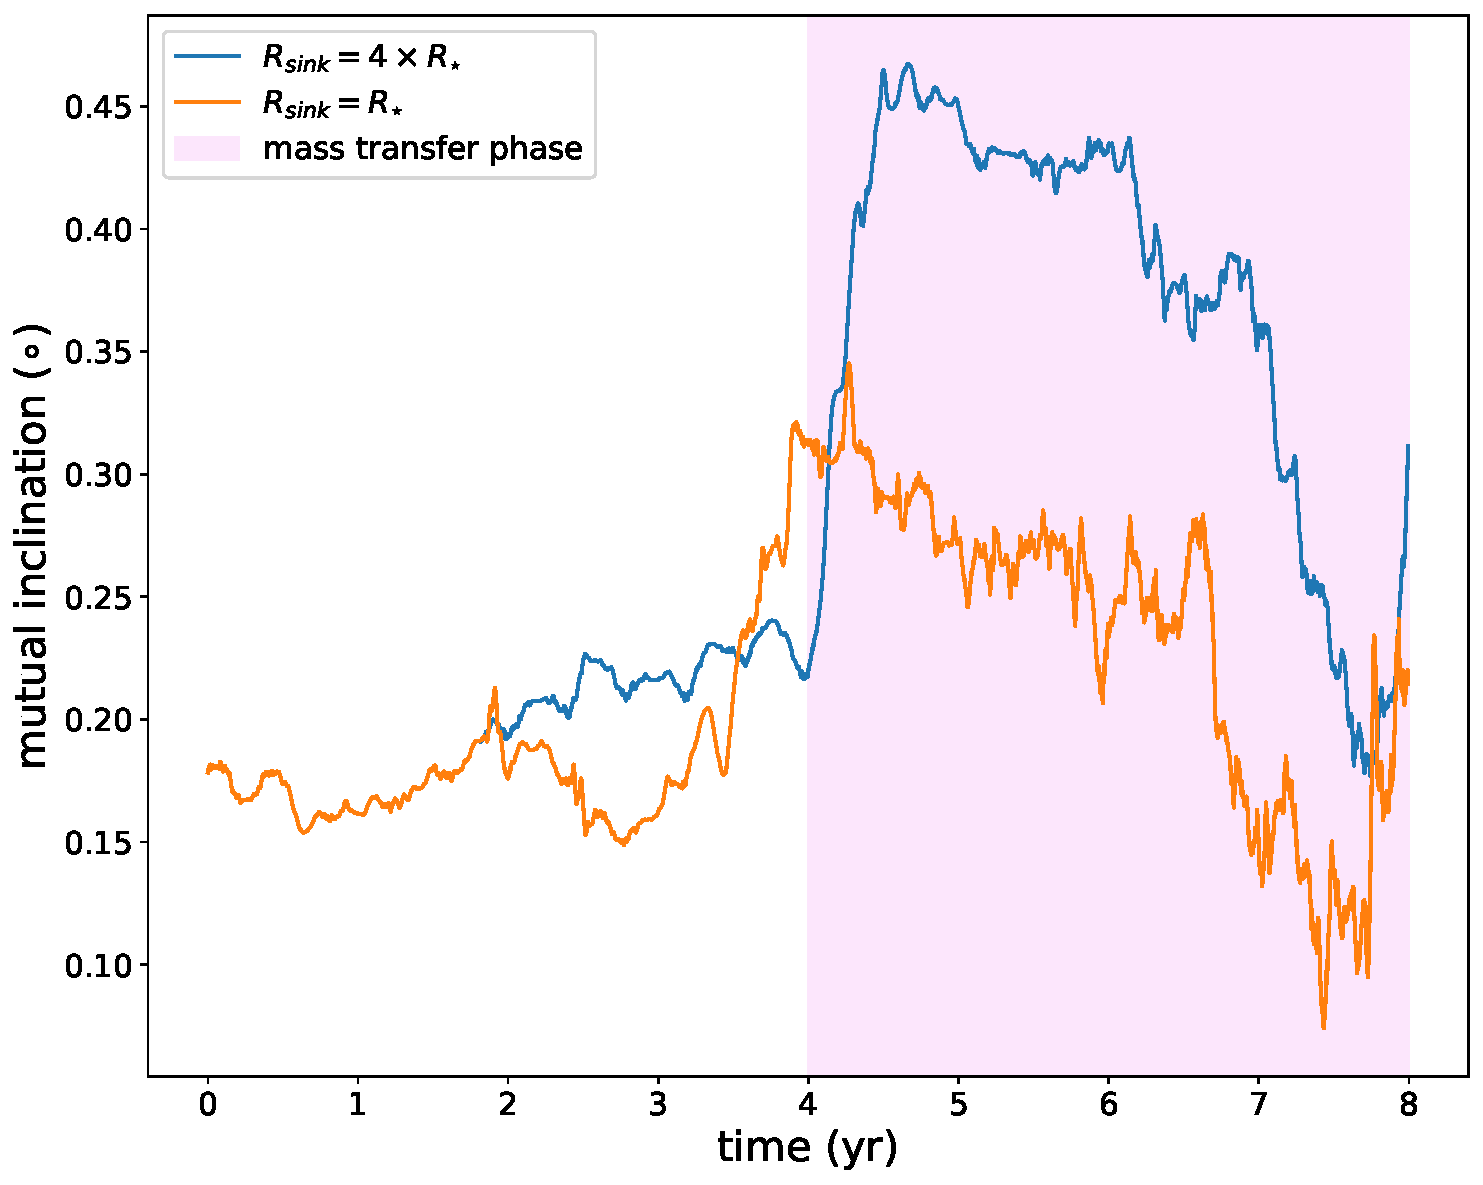
\includegraphics[width=0.8\textwidth]{Thesis/graphs/accretion_case/accretion_inc.pdf}
    \caption{Inclination of the outer orbit relative to the inner orbit.}
    \label{fig:accretion_inc}
\end{figure}
\begin{figure}[H]
    \centering
    \begin{subfigure}{.5\textwidth}
    \centering
    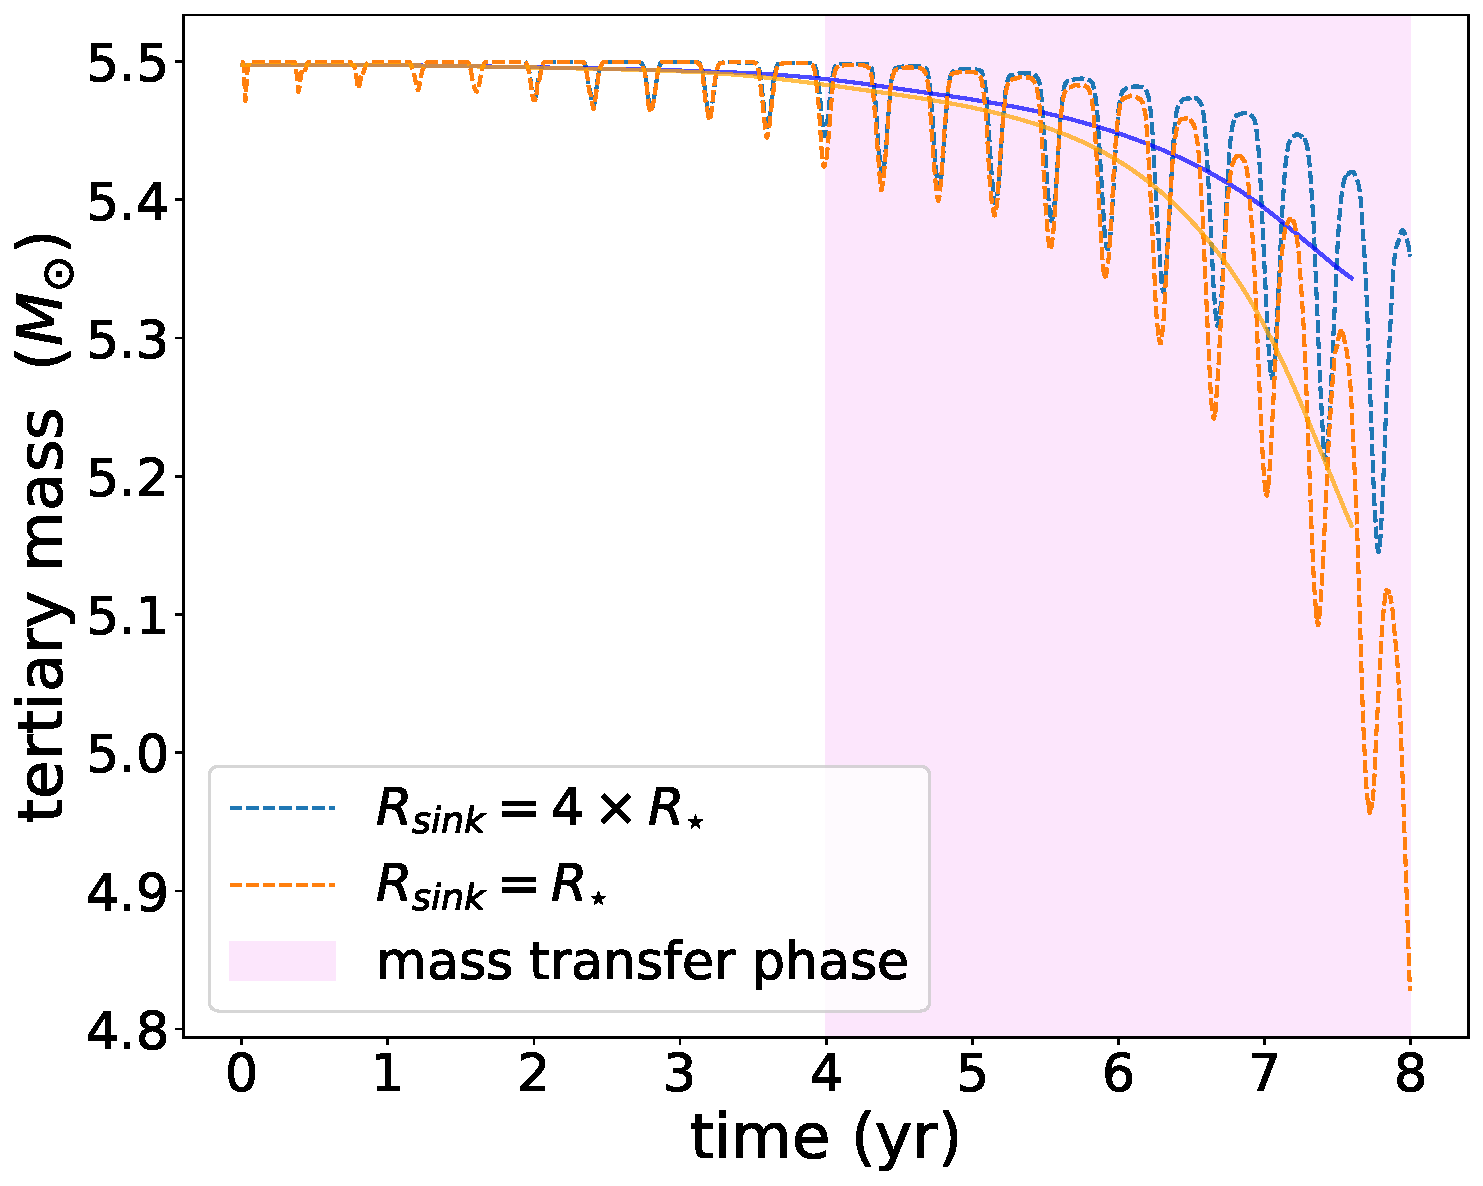
\includegraphics[width=0.9\textwidth]{Thesis/graphs/accretion_case/accretion_mass_loss.pdf}
    \end{subfigure}%
    \begin{subfigure}{.5\textwidth}
    \centering
    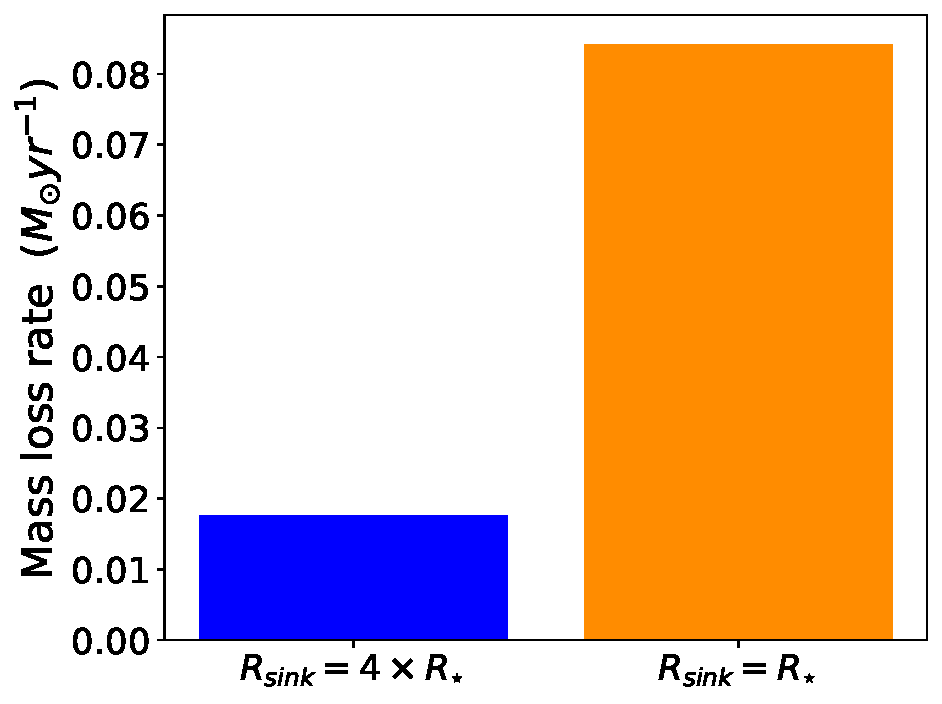
\includegraphics[width=0.9\textwidth]{Thesis/graphs/accretion_case/accretion_giant_mass_loss_rate.pdf}
    \end{subfigure}
    \caption{ The evolution of the tertiary's mass (left) for the minimum and maximum accretion case. The simulated data is shown in dashed lines. The continues lines are smooth representations of the simulated data in their respective colors. The last three orbits are not included in the smoothed version, because the lack of data above $8$ yr will erroneously flatten the slopes. The mean mass loss rates computed using central differentiation on the simulated data (right).}
    \label{fig:accretion_tertiary_mass}
\end{figure}
In \cref{fig:accretion_tertiary_mass}, I present the evolution of the tertiary's mass. The tertiary losses mass much faster in the minimum accretion case. The star's Roche lobe is proportional to its distance from the inner binary's center of mass; see \cref{eq:roche_lobe}, hence as the outer orbit decays faster, see \cref{fig:accretion_outer_semimajor_axis}, the tertiary's Roche lobe shrinks quicker. As a result, more and more gas overflows the Roche lobe and escapes towards the inner binary. To emphasize the difference in the mass evolution, I use central differentiation and provide mean mass loss rates for the simulated period, see \cref{fig:accretion_tertiary_mass}. The mass loss rates, should be taken with a grain of salt. Because the choice of $R_{\star} = 1.1 \times R_L$ significantly overestimates them, they should not be interpreted as real average mass loss rates for RLOF occurring in nature, but they should be treated qualitatively. Despite that, it can not be ignored that the simulated values are in very good agreement with analytical ones calculated using \cref{eq:roche_lobe}.

\subsection{Inner orbit}

In \cref{fig:accretion_inner_semimajor_axis} and \cref{fig:accretion_inner_ecc}, I present the evolution of the semi-major axis and eccentricity of the inner orbit, 
respectively. It is apparent that, the inner orbit widens in both the minimum and maximum accretion case. However, in the minimum accretion case, the orbit widens faster, see \cref{fig:accretion_inner_semimajor_axis}.
\begin{figure}[H]
    \centering
    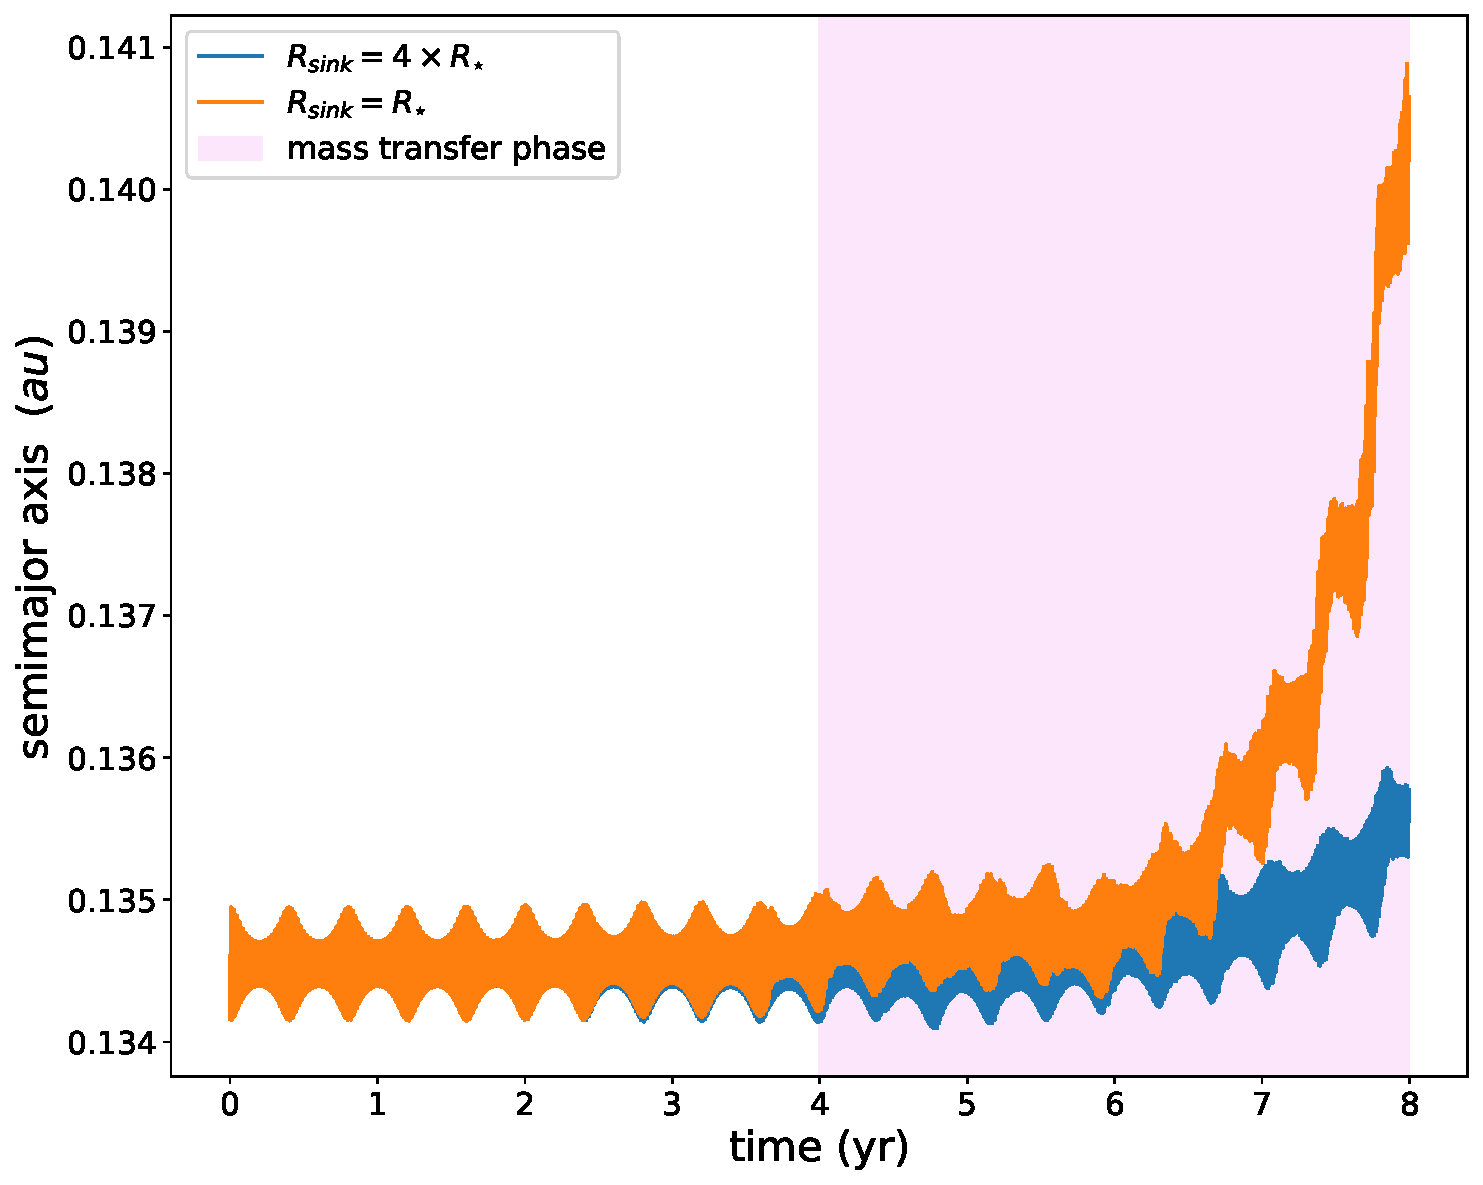
\includegraphics[width=0.9\textwidth]{Thesis/graphs/accretion_case/accretion_inner_semimajor_axis.pdf}
    \caption{Evolution of the semi-major axis of the inner orbit for the minimum and maximum accretion case.}
    \label{fig:accretion_inner_semimajor_axis}
\end{figure}
In the minimum accretion case, the tertiary's mass loss rate is much higher than the maximum accretion case, see \cref{fig:accretion_tertiary_mass} and the aforementioned trend is much more evident. Due to the underestimation of the effect of gas drag, the models are influenced by the gravitational interaction between the binary components and the incoming mass stream. As more mass approaches the binary components, in the minimum accretion case, it can also approach them closer before it is being accreted, increasing the magnitude of the gravitational interactions. In conclusion, it is not possible to confidently draw conclusions about the impact of accretion on the inner orbit's semi-major axis given the current resolution. Finally, as expected, the effect of accretion on the eccentricity of the inner orbit is negligible. The orbit remains circular in both cases.
\begin{figure}[H]
    \centering
    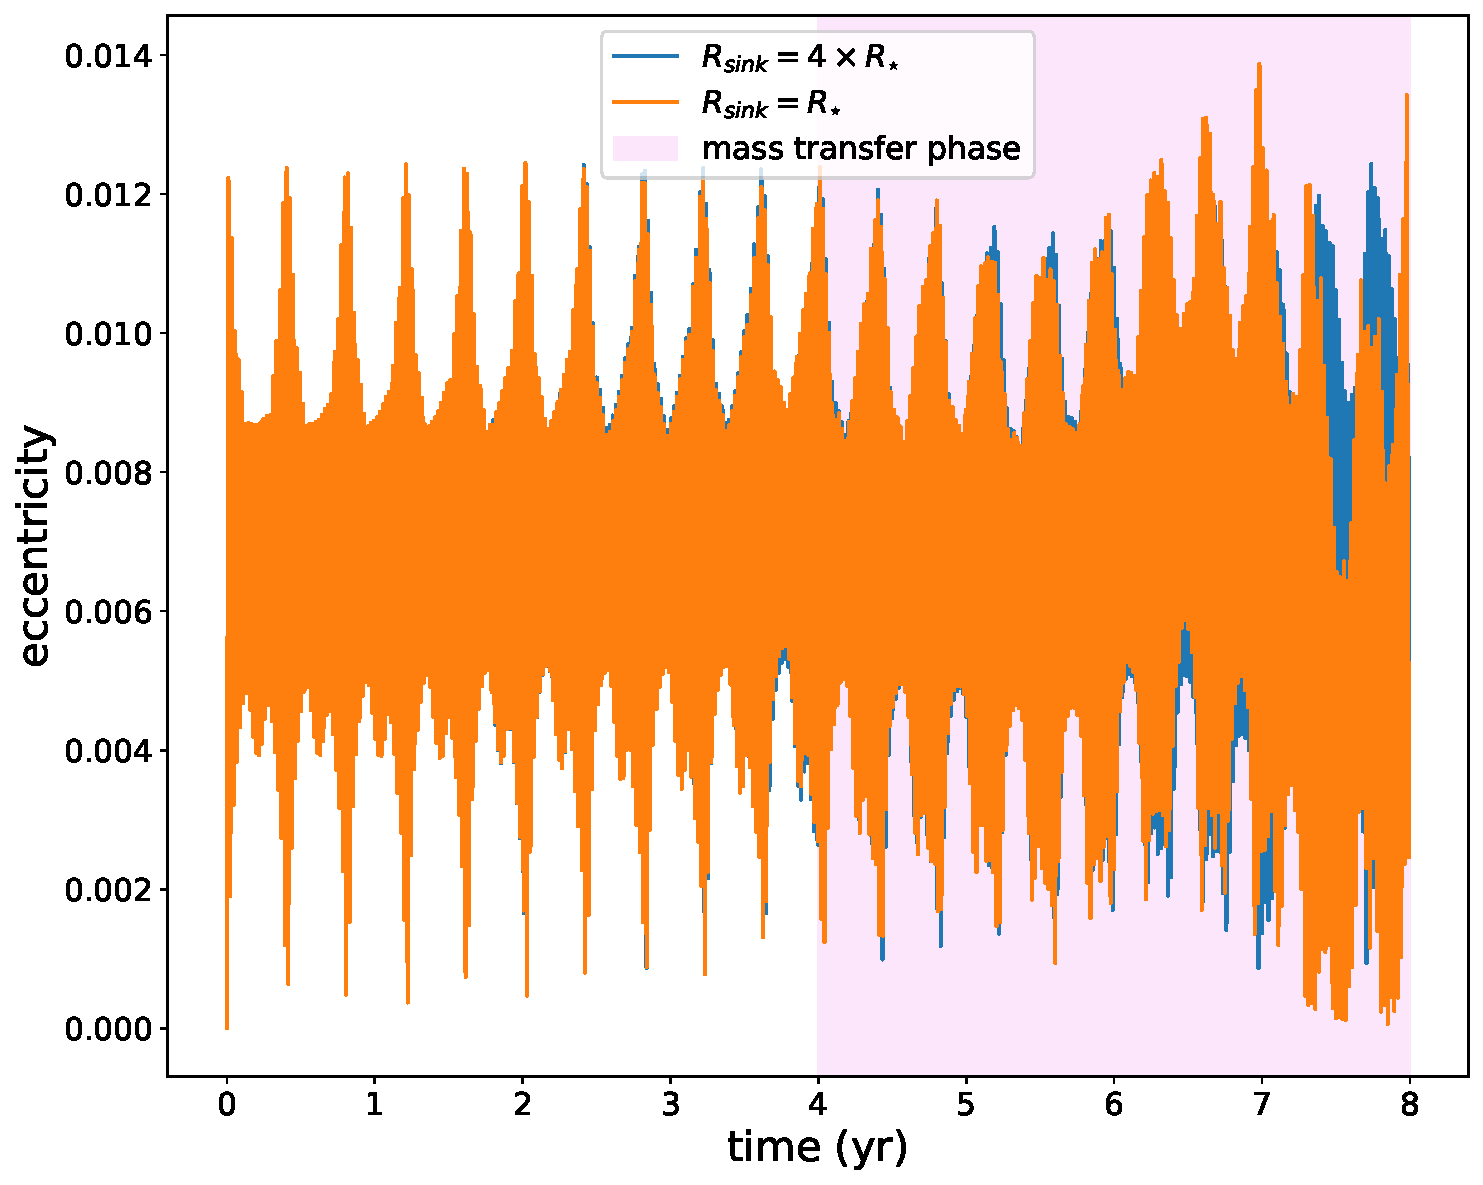
\includegraphics[width=0.9\textwidth]{Thesis/graphs/accretion_case/accretion_inner_ecc.pdf}
    \caption{Evolution of the eccentricity of the inner orbit for the minimum and maximum accretion case.}
    \label{fig:accretion_inner_ecc}
\end{figure}

\subsection{Comparison with analytical model}

During RLOF, matter from the outer donor star is either accreted onto the inner binary stars, forms a disc around them, or is expelled from the triple system entirely. The orbits will change depending on what happens to the mass. This may be expressed in terms of the amount of angular momentum carried by the mass as it exits the donor star. On the one hand, the low resolution of the simulation and thus the underestimation of the gas drag does not allow for a direct comparison between analytical models and the evolution of the inner orbit's semi-major axis. On the other hand, the gas drag on the inner binary is mostly irrelevant for the evolution of the semi-major axis of the outer orbit, thus the amount of the lost angular momentum can be parameterized using analytical models.

In order to get an estimation about how much angular momentum is lost from the system, I compare the evolution of the semi-major axis of the outer orbit with the analytical model based on mass redistribution, see \cref{eq:semimajor_axis_no_cons}. The model assumes conservation of angular momentum despite the non-conservative case, similar to binaries as discussed by \cite{portegies1995formation}. Furthermore, it is assumed that the binary components are orbiting on the same plane, thus I compare the analytical model with the cases where $i_{mut}=0^{\circ}$, see \cref{tab:simulations_settings}.

Due to the fact that one component of the outer orbit is a binary system, the $M_a$ corresponds to its combined mass and $\eta$ is the specific angular momentum of the mass leaving the system as a proportion of the inner binary system's specific angular momentum. 
\begin{figure}[!htb]
    \centering
    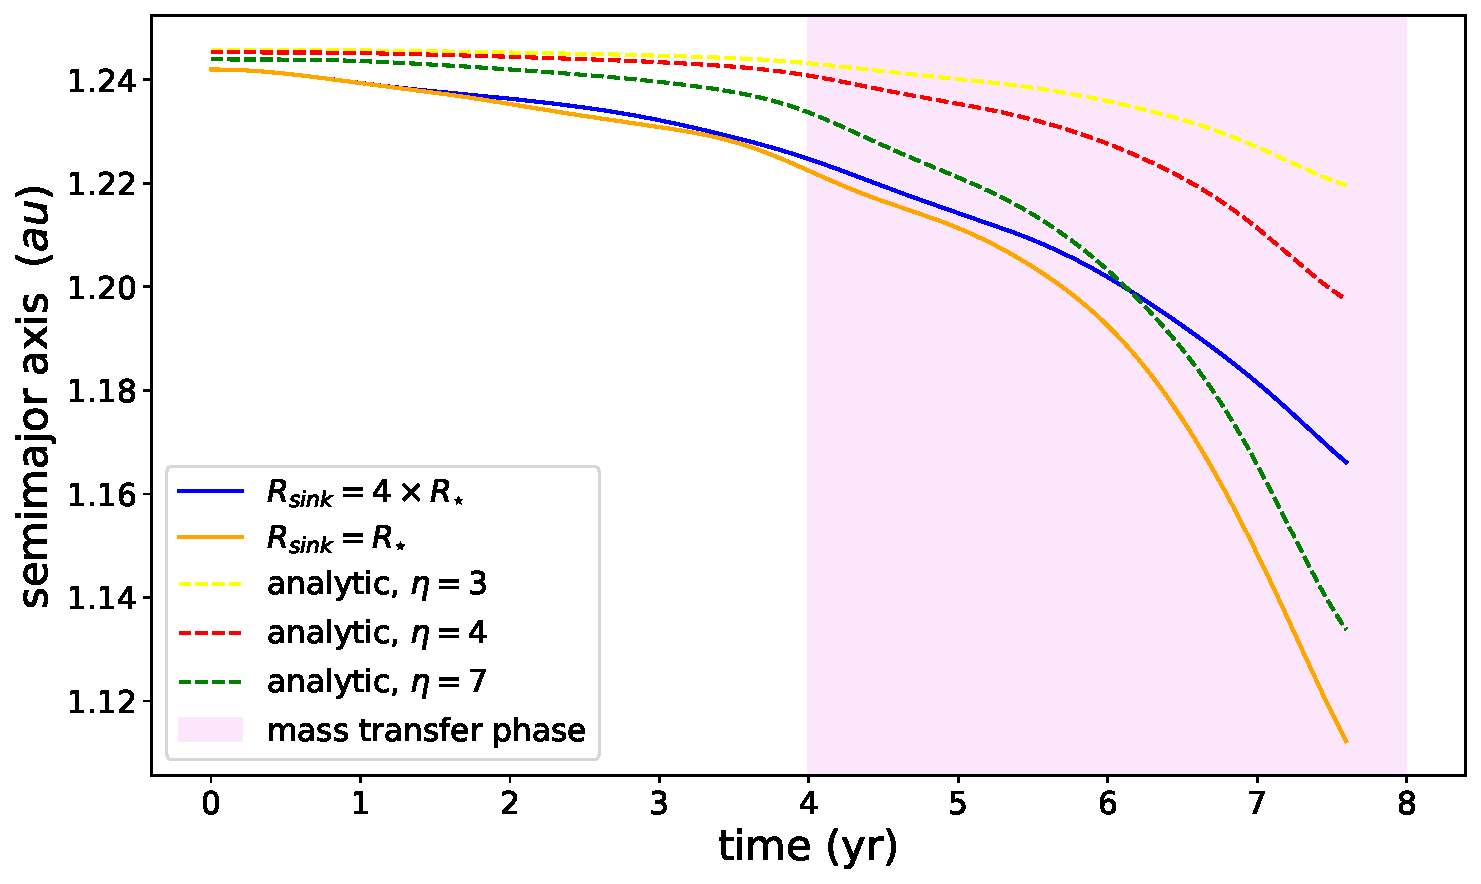
\includegraphics[width=0.85\textwidth]{Thesis/graphs/analytical_model.pdf}
    \caption{Evolution of the semi-major axis of the outer orbit for models number 1 and 4 listed in \cref{tab:simulations_settings}. The continues lines are representations of the simulated data, smoothed with a kernel with width $= 3 \times P_{out}$. The dashed lines correspond to analytical analytical models in yellow, red and green, respectively.  The last three orbits are not included in the smoothed version, because the lack of data above $8$ yr will erroneously flatten the slopes.}
    \label{fig:comparison_analytical_model_max}
\end{figure}
In \cref{fig:comparison_analytical_model_max}, I present  smoothed versions of the simulated data in blue and orange for the maximum and minimum accretion case, respectively. I also overplot three models, based on the maximum accretion case using \cref{eq:semi-major_axis}, for $\eta = 3,4,7$. Higher value of $\eta$ indicate that a higher amount of angular momentum is carried away by the ejected mass. During the mass transfer phase a model with $\eta \approx 4$ matches the slope of the orbital evolution for the maximum accretion case, while a model with $\eta \approx 7$ matches the minimum accretion case's orbital evolution slope. The graph indicates that in the maximum accretion case, given the same amount of ejected mass, the latter should carry significantly more angular momentum in order to match the minimum accretion case ($\eta = 7$). Hence, it is evident that the efficiency of the accretion process is vital for the timescale of the outer orbit's decay.



